% =====================================================================
%  Section IV - Dataset and experimental protocol (HARBox)
%  All numbers come from paper/generated/harbox_*.tex
%  (scripts/tools/paper_harbox_stats.py) or from configs/datasets/harbox.yaml
%  and configs/profiles/harbox*.yaml.
%  The previous Capture-24 version of this section is kept in dataset_capture24.tex.
% =====================================================================
\section{Dataset and Experimental Protocol}\label{sec:data}

% ---------------------------------------------------------------------
\subsection{The HARBox Dataset}\label{sec:data:harbox}

We evaluate on HARBox~\cite{ouyang2021clusterfl}, the largest of the federated HAR datasets
released with ClusterFL. Unlike laboratory collections, it was \emph{crowd-sourced}: volunteers
installed an Android application on their own smartphones and recorded five activities of daily
life, labelling each recording themselves by pressing ``start'' and ``end'' in the
application (\cref{tab:classes}). After invalid and repeated submissions were removed, the data
of $121$ users aged $17$--$55$ years remained, recorded with $77$ different smartphone models. Each
recording contains the $9$-axis inertial signals of the phone (tri-axial accelerometer in
m\,s$^{-2}$, gyroscope in rad\,s$^{-1}$ and magnetometer in $\mu$T), resampled by the authors to
$50$\,Hz and cut into $2$\,s windows with a $1$\,s hop, so consecutive windows of a recording
overlap by $50\,\%$. One user has no windows. The remaining $\HBUsers{}$ users contribute
$\HBWindows{}$ windows (about $\HBHours{}$\,h of distinct signal). Users and phones are the natural
unit of federation, so every user is one client and no synthetic partition is needed. The
heterogeneity that federated HAR must handle (different devices, grips, body sizes and
movement styles) is present by construction.

\begin{table}[!t]
\centering
\caption{HARBox activities after windowing ($2$\,s windows, $50$\,Hz, $9$ axes), over all
\HBUsers{} users. Users: users with at least one window of the activity.}
\label{tab:classes}
\footnotesize
\setlength{\tabcolsep}{4pt}
\renewcommand{\arraystretch}{1.1}
\begin{tabularx}{\columnwidth}{@{}l Y r r r@{}}
\toprule
Activity & Description & Windows & \% & Users \\
\midrule
\inputrows{generated/harbox_tab_classes.tex}
\bottomrule
\end{tabularx}
\end{table}

\begin{figure*}[!t]
  \centering
  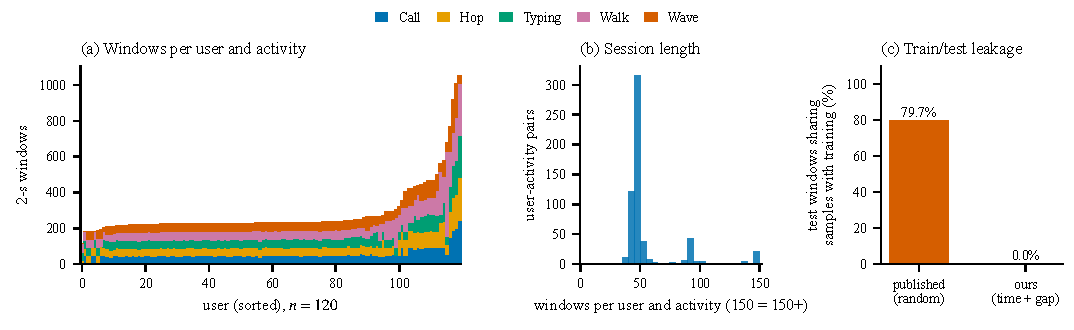
\includegraphics[width=\textwidth]{figures/harbox_stats.pdf}
  \caption{HARBox at a glance. (a)~Windows per user and activity: users differ in how long they
  recorded, not in which activities. (b)~Length of the recording of one activity by one user,
  typically below one minute. (c)~Share of test windows that overlap a training window by half of
  their samples. The random split of the published protocol leaks the large majority; our
  per-activity chronological split with a one-window gap leaks none.}
  \label{fig:harbox}
\end{figure*}

% ---------------------------------------------------------------------
\subsection{Preprocessing}\label{sec:data:preprocessing}

We use the windows exactly as released: each window is a $9\times100$ array in physical units,
ordered by its start time, and assigned the activity of the file it comes from. We also
reconstruct the recording session of each window from the timestamps: a new session starts
wherever two consecutive windows of an activity start more than $1.5$\,s apart. The median user
contributes $\HBWinUserClassMedian{}$ windows per activity, i.e., less than one minute of
recording, in a median of five sessions. No resampling or filtering is applied at storage time.
The encoder-specific preprocessing $\Pi_E$ (\cref{sec:method:client}) converts units, resamples to
the encoder's rate and fits the window length (\cref{tab:encoders}). Only the training windows
are augmented (\cref{sec:data:impl}).

% ---------------------------------------------------------------------
\subsection{Evaluation Protocols}\label{sec:data:splits}

Two protocols are used (\cref{tab:partition}).

\emph{Protocol A (published).} To compare with published results, we reproduce the protocol of
FedCHAR~\cite{li2023fedchar}: every user is a client, draws a random number of $50$ to $500$ of its
windows, and splits them at random into $72\,\%$ training, $8\,\%$ validation and $20\,\%$ test
windows. Training runs for $100$ rounds with half of the users per round, and the metric is the
mean test accuracy over users. Because consecutive windows overlap by $50\,\%$, however, a random
split places at least one neighbour of most test windows in the training set. We measured that
$\HBLeakA\,\%$ of the test windows share half of their samples with a training window
(\cref{fig:harbox}c). Protocol~A therefore rewards memorizing a user's recordings rather than
recognizing the activity, and we use it only for the comparison with published numbers.

\emph{Protocol B (ours, leakage-free).} The $\HBUsers$ users are randomly assigned, with a fixed
seed, to $\HBClientsB$ FL clients ($70\,\%$), $\HBHeldoutB$ held-out users ($20\,\%$) and $\HBPoolB$
pool users ($10\,\%$). Every activity of a client is split \emph{in time}: the first $80\,\%$ of its
windows are used for training and the last $20\,\%$ for testing. The window between the two
parts is discarded, because it overlaps both. A plain chronological split of the whole recording
would put entire activities into the test part, since HARBox records each activity in its own
session. No test window overlaps a training window, and every activity of a client appears on
both sides. The held-out users never take part in training. For each of their activities, the
first half is the pool from which few-shot labels may be drawn and the second half is the test
set (again with a one-window gap). The pool users provide unlabelled data for the
self-supervised pretraining of HALO and serve as validation users for model selection. No test
data are used for any choice. All main results of this paper use Protocol~B. LIMU-BERT and the MLP
baselines are repeated on two further user splits (seeds $1$ and $2$, \cref{tab:seeds}).

\begin{table}[!t]
\centering
\caption{The two evaluation protocols on HARBox (seed $0$). $^{\dagger}$Pool users' windows (validation).}
\label{tab:partition}
\footnotesize
\setlength{\tabcolsep}{3pt}
\renewcommand{\arraystretch}{1.12}
\begin{tabularx}{\columnwidth}{@{}>{\raggedright\arraybackslash}p{2.3cm} Y Y@{}}
\toprule
 & Protocol B (ours) & Protocol A (published) \\
\midrule
\inputrows{generated/harbox_tab_partition.tex}
\bottomrule
\end{tabularx}
\end{table}

% ---------------------------------------------------------------------
\subsection{Statistical Heterogeneity}\label{sec:data:hetero}

HARBox differs from free-living datasets in where its heterogeneity lies (\cref{tab:hetero}).
Label skew is mild: $112$ of the $\HBUsers$ users recorded all five activities, and a user's
label distribution diverges from the global one by only $\HBJSD$ bits on average. Quantity skew is
substantial ($\HBWinUserMin$ to $\HBWinUserMax$ windows per user). The dominant heterogeneity is in
the signals themselves. Seventy-seven phone models with different sensor ranges, noise levels and
axis conventions are held, pocketed and waved by $\HBUsers$ different people, each recording every
activity only once and for less than a minute. The class-conditional distributions
$p_k(\mathbf{x}\mid y)$ therefore differ strongly between users (heterogeneity~(H2) in
\cref{sec:method:problem}), and they can be learned only from very little data per user. This is
the regime that the local normalization, the local input adapter and the personal classifier of
\method{} are designed for. The label-skew remedies of \cref{sec:method:skew} matter less here.

\begin{table}[!t]
\centering
\caption{Statistical heterogeneity of the \HBUsers{} HARBox users. JSD: Jensen--Shannon divergence in bits.}
\label{tab:hetero}
\footnotesize
\renewcommand{\arraystretch}{1.1}
\begin{tabularx}{\columnwidth}{@{}Y r@{}}
\toprule
Statistic & Value \\
\midrule
\inputrows{generated/harbox_tab_hetero.tex}
\bottomrule
\end{tabularx}
\end{table}

% ---------------------------------------------------------------------
\subsection{Pretrained Encoders}\label{sec:data:encoders}

To test whether the conclusions depend on the backbone, we instantiate \method{} with four IMU
encoders that differ in architecture (Transformer, residual CNN, spatio-temporal graph network,
patch-channel Transformer), size ($51$\,k to $10.4$\,M frozen parameters), pretraining corpus and
objective, and input format (\cref{tab:encoders}). We add the multilayer perceptron of the published
HARBox results~\cite{ouyang2021clusterfl,li2023fedchar} as a from-scratch reference. Three encoders use their official
checkpoints, loaded into re-implementations with identical parameter names (loading fails if
less than $90\,\%$ of the tensors match). LIMU-BERT was pretrained on smartphone data with
accelerometer and gyroscope~\cite{stisen2015smart}, the closest match to HARBox. Its 120 position
embeddings cover $6$\,s at $20$\,Hz, of which a $2$\,s window uses the first $40$. ssl-wearables expects
$10$\,s at $30$\,Hz, so the resampled $2$\,s window is repeated five times. UniMTS receives the
accelerometer on the right-wrist joint of its 22-joint skeleton, the joint closest to a
hand-held phone. HALO~\cite{ding2026halo} has not released weights. We re-implemented its encoder at a
reduced width ($d=192$) and pretrained it with its stage-1 objectives (masked reconstruction of
$50\,\%$ of the patches~\cite{he2022masked} and a patch-level InfoNCE loss~\cite{oord2018representation})
on the unlabelled windows of the pool users, with all nine axes and $0.4$\,s patches. Because HALO
tokenizes every channel separately, it is the only pretrained encoder that uses the magnetometer
from the start. The input adapters of the others may learn to mix it in.

\begin{table*}[!t]
\centering
\caption{Encoders and their HARBox input. Input: channels after the input adapter, sampling
rate, samples (duration) and units, produced from the stored $9\times100$ window by $\Pi_E$.}
\label{tab:encoders}
\footnotesize
\setlength{\tabcolsep}{4pt}
\renewcommand{\arraystretch}{1.15}
\begin{tabularx}{\textwidth}{@{}l Y Y l r r@{}}
\toprule
Encoder & Architecture & Pretraining data and objective & HARBox input & $d_z$ & $|\Omega_0|$ \\
\midrule
LIMU-BERT~\cite{xu2021limubert} &
  Transformer, 4 weight-shared layers (ALBERT-style), $d=72$, 4 heads, mean pooling &
  HHAR smartphones and smartwatches~\cite{stisen2015smart}; masked-span reconstruction (official checkpoint) &
  6 (acc+gyro), 20\,Hz, 40 (2\,s), $g$ & 72 & 51\,k \\
ssl-wearables~\cite{yuan2024selfsupervised} &
  1-D ResNet-V2 (harnet10), 5 stages, 64--1024 channels, anti-aliased down-sampling &
  UK Biobank, 700\,k person-days of wrist accelerometry; multi-task self-supervision &
  3 (acc), 30\,Hz, 60 tiled to 300, $g$ & 1024 & 10.4\,M \\
UniMTS~\cite{zhang2024unimts} &
  ST-GCN~\cite{yan2018spatial}, 10 blocks over a 22-joint skeleton graph, 64--512 channels &
  IMU synthesized from motion capture (HumanML3D~\cite{guo2022generating}); contrastive text alignment &
  3 (acc) on wrist joint, 20\,Hz, 40, m\,s$^{-2}$ & 512 & 5.2\,M \\
HALO~\cite{ding2026halo} (re-impl.) &
  0.4-s patch $\times$ channel tokens, 8 alternating temporal/cross-channel attention layers, $d=192$, query pooling &
  HARBox pool users (unlabelled, disjoint from all evaluation users); masked reconstruction + patch contrastive &
  9 (acc+gyro+mag), 50\,Hz, 100, $g$ & 256 & 4.6\,M \\
MLP~\cite{li2023fedchar} &
  flattened window, one hidden layer of 300 units (the published HARBox model) &
  none (trained from scratch) &
  9, 50\,Hz, 100 (900 features) & 300 & -- \\
\bottomrule
\end{tabularx}
\end{table*}

% ---------------------------------------------------------------------
\subsection{Compared Methods}\label{sec:data:methods}

\Cref{tab:methods} lists the federated methods, each defined by the roles of \cref{tab:roles}.
FedAvg trains the whole model from a random initialization. V0 and V1 are the upper-cost and
lower-cost ways of using a pretrained encoder (full fine-tuning; a frozen encoder with trainable
heads). V2 and V3 isolate the aggregation rule for homogeneous LoRA: factor averaging versus
exact aggregation~\cite{singhal2025fedex}. V4 adds rank heterogeneity with the delta-form
aggregation of \cref{sec:method:agg}, and it is the ablation of \method{} (V5) without local parts and
prototypes. The MLP is trained with the baselines of the published HARBox results: FedAvg, purely
local training, and Ditto~\cite{li2021ditto}, the personalized method on which FedCHAR
builds. Because Ditto is the strongest of these, we also run it from the pretrained LIMU-BERT
(Ditto, pretrained), which gives the personalized full-model baseline at the communication cost of
V0. Every method uses the same augmentation, decoders and evaluation. Two centralized
references are trained on the pooled training parts of the clients: \emph{from scratch}, which
defines the target accuracy, and \emph{pretrained fine-tuning}, an upper reference without privacy
constraints.

\begin{table*}[!t]
\centering
\caption{Federated methods. $\Omega$: encoder weights; $g$, $h$: shared and classifier heads;
$\psi$: normalization; $a$: input adapter; P: prototypes.}
\label{tab:methods}
\footnotesize
\setlength{\tabcolsep}{4.5pt}
\renewcommand{\arraystretch}{1.12}
\begin{tabular}{@{}l l l l l l l@{}}
\toprule
Method & Init. & Trained & Uploaded & Kept local & LoRA rank & Aggregation \\
\midrule
Local & random & $\Omega,\psi,a,g,h$ & -- & everything & -- & none \\
FedAvg~\cite{mcmahan2017fedavg} & random & $\Omega,\psi,a,g,h$ & $\Omega,\psi,a,g,h$ & -- & -- & FedAvg \\
Ditto~\cite{li2021ditto} & random & global + personal copy & $\Omega,\psi,a,g,h$ & personal copy & -- & FedAvg + proximal personal model \\
V0 Full fine-tuning & pretrained & $\Omega,\psi,a,g,h$ & $\Omega,\psi,a,g,h$ & -- & -- & FedAvg \\
Ditto, pretrained & pretrained & global + personal copy & $\Omega,\psi,a,g,h$ & personal copy & -- & FedAvg + proximal personal model \\
V1 Head only & pretrained & $g,h$ & $g,h$ & -- & -- & FedAvg \\
V2 LoRA, factor averaging & pretrained & LoRA, $g,h$ & LoRA, $g,h$ & -- & 8 & avg.\ $A$, avg.\ $B$ \\
V3 LoRA, exact & pretrained & LoRA, $g,h$ & LoRA, $g,h$ & -- & 8 & FedEx-LoRA~\cite{singhal2025fedex} \\
V4 Heterogeneous ranks & pretrained & LoRA, $g,h$ & LoRA, $g,h$ & -- & 2/4/8 & delta form + SVD (\cref{sec:method:agg}) \\
\textbf{V5 \method} & pretrained & LoRA, $g,h,\psi,a$ & LoRA, $g$, P & $h,\psi,a$ & 2/4/8 & delta form + SVD, prototypes \\
\bottomrule
\end{tabular}
\end{table*}

% ---------------------------------------------------------------------
\subsection{Evaluation Metrics}\label{sec:data:metrics}

\emph{Recognition.} Following the published HARBox results, the primary metric is the \emph{mean
per-user accuracy}, i.e., the test accuracy of every client averaged over clients. We also report
the macro-F1 over the five activities, computed on the pooled test windows of all clients.

\emph{Fairness.} We report the mean accuracy of the $\lceil0.1K\rceil$ worst-served clients
(\emph{worst-10\,\%}) and the standard deviation of the per-client macro-F1 over the activities
present in each client's test part.

\emph{Communication.} Every message is an explicit set of tensors whose size is measured as the
serialized size of uncompressed arrays (four bytes per real value, eight per integer), as in
Flower's NumPy serialization~\cite{beutel2020flower}. It includes every tensor that is sent:
factors, heads, residual weights, prototypes and counts. We report the uplink per client update
(MB), the rounds to target (the first evaluated round whose macro-F1 reaches $90\,\%$ of the
centralized from-scratch macro-F1 of the same encoder) and the cumulative uplink up to that round.
No compression or quantization is applied.

\emph{Client cost.} The client memory is the size of all model tensors plus the peak additional
device memory allocated during a local update, measured with the CUDA allocator. The client time
is the wall-clock time of one local update.

\emph{New users (Protocol B).} On the \HBHeldoutB{} held-out users we report the mean per-user
macro-F1 on their test parts: zero-shot (no labels) and few-shot with $1$, $5$ and $10$ labelled
windows ($2$, $10$ and $20$\,s) per activity, drawn at random from their adaptation parts.

\emph{Personalized evaluation.} Methods with a shared classifier are also scored after the common
``FedAvg + local fine-tuning'' step (``+FT''): every client fine-tunes only the classifier on its
own training part ($20$ steps) and is scored with it. Local, Ditto and \method{} are personal by
design. Temporal decoding (\cref{sec:method:inference}) is not used on HARBox: every activity is
recorded in its own session, so a sequence model would only learn that the label never changes
within a recording.

% ---------------------------------------------------------------------
\subsection{Implementation Details}\label{sec:data:impl}

All methods run in one transparent federated simulator written in PyTorch~2.11 (Python~3.13).
All windows reside in GPU memory, so a mini-batch is an index tensor and every method sees
exactly the same data stream for a given seed. Experiments ran on a single NVIDIA GeForce
GTX~1660~Ti (6\,GB) in fp32. \Cref{tab:hparams} lists the hyperparameters. Because the $77$ phone
models are held in many different ways, every training window of every method is augmented with
probability $0.8$ by one random rotation of up to $30^\circ$, applied jointly to the accelerometer,
gyroscope and magnetometer triplets, and by a random gain ($\mathcal{N}(1,0.1^2)$). The three large
encoders are $5$--$15$ times slower per step than LIMU-BERT on this GPU and therefore train with a
reduced budget (\cref{tab:hparams}). All methods of an encoder share its budget, so methods are
comparable within an encoder. All local updates use AdamW~\cite{loshchilov2019adamw} with a fresh
optimizer state in every round.

\begin{table}[!t]
\centering
\caption{Hyperparameters on HARBox (Protocol B unless stated). Budget of ssl-wearables and HALO / UniMTS in parentheses where it differs.}
\label{tab:hparams}
\footnotesize
\setlength{\tabcolsep}{3pt}
\renewcommand{\arraystretch}{1.08}
\begin{tabularx}{\columnwidth}{@{}l Y@{}}
\toprule
\multicolumn{2}{@{}l}{\textit{Federated training}} \\
Rounds $T$; clients per round & $100$ ($60$ / $40$); $17$ of $84$ ($\rho=0.2$) \\
Local work per round & $2$ epochs, capped at $8$ ($6$ / $4$) steps of batch $64$ \\
Learning rates & FedAvg $10^{-3}$; V0 body $3\!\times\!10^{-4}$; LoRA, heads, $\psi$, $a$: $2\!\times\!10^{-3}$ \\
Weight decay & $10^{-4}$ \\
LoRA & $r=8$ (V2, V3); tiers $\{2,4,8\}$ uniform (V4, V5); $\alpha=2r$; dropout $0$ \\
Embedding $D$; prototype weight $\lambda$ & $64$; $0.5$ (prototypes on $\le512$ windows) \\
Shared classifiers & $\tau=1$ with client prior; class-wise rows; $\tau_{\mathrm{inf}}=0.5$ \\
Ditto & proximal weight $0.1$ \\
Augmentation & rotation $\le30^\circ$ (acc, gyro, mag jointly), gain $\mathcal{N}(1,0.1^2)$, $p=0.8$ \\
Final personalization; +FT & $20$ steps on $\phi_k$; $20$ steps on $h$ \\
\midrule
\multicolumn{2}{@{}l}{\textit{New users}} \\
Few-shot labels; steps & $1$, $5$, $10$ windows per activity; $60$ ($30$ for UniMTS) \\
\midrule
\multicolumn{2}{@{}l}{\textit{Centralized references}} \\
Epochs; early stopping & $25$ ($20$ / $15$, UniMTS $8{,}000$ windows per epoch), cosine; patience $5$ \\
Batch; learning rate & $128$ (UniMTS $64$); scratch $10^{-3}$, fine-tuning $3\!\times\!10^{-4}$ \\
\midrule
\multicolumn{2}{@{}l}{\textit{HALO pretraining (pool users)}} \\
Schedule & $40$ epochs, batch $128$, AdamW lr $3\!\times\!10^{-4}$ (cosine) \\
\midrule
\multicolumn{2}{@{}l}{\textit{Protocol A (published)}} \\
Clients; rounds & all $120$ users, $50\,\%$ per round; $100$ rounds \\
MLP baselines & $5$ local epochs, batch $32$ (as published) \\
\bottomrule
\end{tabularx}
\end{table}
